%%%%%%%% ICML 2019 EXAMPLE LATEX SUBMISSION FILE %%%%%%%%%%%%%%%%%

\documentclass{article}

% Recommended, but optional, packages for figures and better typesetting:
\usepackage{microtype}
\usepackage{graphicx}
\usepackage{subfigure}
\usepackage{booktabs} % for professional tables
\usepackage{amsmath}

% hyperref makes hyperlinks in the resulting PDF.
% If your build breaks (sometimes temporarily if a hyperlink spans a page)
% please comment out the following usepackage line and replace
% \usepackage{icml2019} with \usepackage[nohyperref]{icml2019} above.
\usepackage{hyperref}

% Attempt to make hyperref and algorithmic work together better:
\newcommand{\theHalgorithm}{\arabic{algorithm}}

% Use the following line for the initial blind version submitted for review:
\usepackage{icml2019}[accepted]

% If accepted, instead use the following line for the camera-ready submission:
%\usepackage[accepted]{icml2019}

% The \icmltitle you define below is probably too long as a header.
% Therefore, a short form for the running title is supplied here:
\icmltitlerunning{Kaggle Galaxy Zoo Clustering using Deep Embedding Clustering}

\begin{document}

\twocolumn[
\icmltitle{Kaggle Galaxy Zoo Image Data Clustering \\
	      using Deep Embedding Clustering}

% It is OKAY to include author information, even for blind
% submissions: the style file will automatically remove it for you
% unless you've provided the [accepted] option to the icml2019
% package.

% List of affiliations: The first argument should be a (short)
% identifier you will use later to specify author affiliations
% Academic affiliations should list Department, University, City, Region, Country
% Industry affiliations should list Company, City, Region, Country

% You can specify symbols, otherwise they are numbered in order.
% Ideally, you should not use this facility. Affiliations will be numbered
% in order of appearance and this is the preferred way.
\icmlsetsymbol{equal}{*}

\begin{icmlauthorlist}
\icmlauthor{Saksham Goel}{umn}
\end{icmlauthorlist}

\icmlaffiliation{umn}{Computer Science & Engineering, University of Minnesota Twin-Cities, Minneapolis, USA}

% You may provide any keywords that you
% find helpful for describing your paper; these are used to populate
% the "keywords" metadata in the PDF but will not be shown in the document
\icmlkeywords{Machine Learning, ICML}

\vskip 0.3in
]

% this must go after the closing bracket ] following \twocolumn[ ...

% This command actually creates the footnote in the first column
% listing the affiliations and the copyright notice.
% The command takes one argument, which is text to display at the start of the footnote.
% The \icmlEqualContribution command is standard text for equal contribution.
% Remove it (just {}) if you do not need this facility.

%\printAffiliationsAndNotice{}  % leave blank if no need to mention equal contribution
\printAffiliationsAndNotice{\icmlEqualContribution} % otherwise use the standard text.





%%%%%%%%%%%%%%%%%%%%%%%%%%%%%%%%%%%%%%%%%%%%%%%%%%%%%%%%%%%%%%%%%%%%%%%
% ABSTRACT %
%%%%%%%%%%%%%%%%%%%%%%%%%%%%%%%%%%%%%%%%%%%%%%%%%%%%%%%%%%%%%%%%%%%%%%%
\begin{abstract}
Galaxies are one of the most fundamental entity of the universe. They come in all shapes, sizes and colors and 
in order to understand how the different shapes (or morphologies) of these galaxies relate to the physics that 
create them it is important to group similar galaxies based on their structure. Considering the number of galaxy 
images collected through numerous telescopes this project tries to evaluate the performance of a proposed deep 
neural network architecture using Convolutional Neural Networks as feature extractor for clustering based of the 
algorithm: \textbf{``Deep Embedding Clustering"} \cite{dec} over a simple DEC based clustering network architecture
 on the Kaggle Galaxy Zoo data. The performance of the algorithm 
is evaluated based on the separation of \textit{``Elliptical"} and \textit{``Spiral"} galaxy images into distinct clusters.
\end{abstract}
%%%%%%%%%%%%%%%%%%%%%%%%%%%%%%%%%%%%%%%%%%%%%%%%%%%%%%%%%%%%%%%%%%%%%%%
%%%%%%%%%%%%%%%%%%%%%%%%%%%%%%%%%%%%%%%%%%%%%%%%%%%%%%%%%%%%%%%%%%%%%%%

















%%%%%%%%%%%%%%%%%%%%%%%%%%%%%%%%%%%%%%%%%%%%%%%%%%%%%%%%%%%%%%%%%%%%%%%
% Introduction %
%%%%%%%%%%%%%%%%%%%%%%%%%%%%%%%%%%%%%%%%%%%%%%%%%%%%%%%%%%%%%%%%%%%%%%%
\section{Introduction}
\label{introduction}
Understanding how and why we are here is one of the fundamental questions for the human race. In the quest of understand our origin we as human race also realized how important it is to understand the origin of our universe and all of its entities. According to many scientists galaxies, the most fundamental entity of the universe, might just hold the answer about the origin and evolution of the universe. Galaxies are of very different forms, size and shapes which has led scienties to believe that the inherent structure of galaxies might hold the clue to understanding the laws of physics that govern our universe. This quest for answers is what led to space exploration and development of thousands of telescopes to capture snapshots of galaxies in an effort to understand the structure of the galaxies and how it is critical to the origin and evolution of the universe itself. However in each passing moment, telescopes are capturing more and more images of galaxies far far away. Few decades ago the scientific community depended on massive citizen science crowdsourcing projects ((INSERT CITATION)) to help identofy the type of galaxies in each of the images captured. However because of the recent explosion in the number of images around million or even billions of images, it is virtually impossible for the community to depend on the citizen science projects to label each image individually. 

To combat this problem the community pivoted to well establised Supervised Deep Learning techniques using Convolutional Neural Networks (CNN) for classifying each galaxy image and help in labelling the huge dataset. However, supervised learning deep learning techniqes are very much like a black box that takes in an input and returns an output, which in this case is just an image and a class label respectivesl. Using these models thus does not help understand what features define these galaxies and how do the inherent structure help in identifying the type of galaxy the image belongs to.  Also the perfomance of some of these models   decrease when tested on new images being captured. Because of this problem the community has to contnuously train these models which require volunteer labels for new images and thus leads to the same problem. 

To address this problem, \textbf{Zooniverse} ((INSERT CITATION)) another citizen science crowdsourcing project has developed techniques which rely on clusters of images to efficiently collect labels for many images in much less time. Also using a clustering based approach helps in understanding what features of the galaxy are most influential and how do the structure relate to the galaxy type. Apart from that using clustering technique helps in extracting information about the most representative structure of the galaxies along with information about the similarity among galaxies of the same type. This experiment is part of their project to develop a more sophisticated technique which is able to cluster similar type of galaxy images together. The new galaxy clustering algorithm is based off a proposed architecture that uses a pretrained Convolutional Neural Network as a feature extractor along with the \textbf{``Deep Embedding Clustering (DEC)"} \cite{dec} architecture that helps to cluster the galaxy images. The motivation for this architecture comes from the recent advances in the development of CNN based image extractors and their proven performance in image classification tasks \cite{imagenet}, along with the results of the DEC architecture in succesfully clustering the MNIST \cite{mnist} and REUTERS \cite{reuters} dataset. In this experiment we evaluate the performance of the proposed architecture over the performance of a standalone DEC architecture over the publicly available Kaggle Galaxy-Zoo dataset. For this experiment we are just evaluating the performance of the architecture on 2 classes of the galaxies which are: ``Elliptical" and ``Spiral". The size of the images in dataset is 424 by 424. An example of each of these galaxy images is provided in: Figure: \ref{galaxy_examples}. 

\begin{figure}[ht]
\vskip 0.2in
\begin{center}
\centering
  \subfigure[Spiral Galaxy]{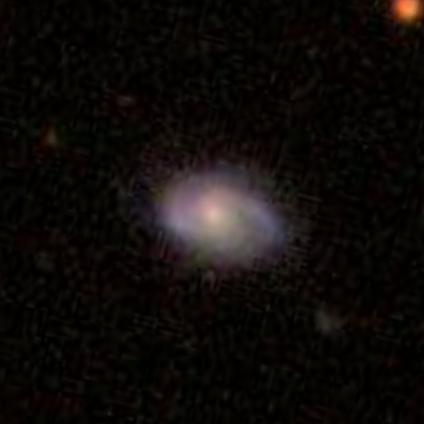
\includegraphics[scale=0.3]{figs/galaxies/spiral.jpg}}\quad
  \subfigure[Elliptical Galaxy]{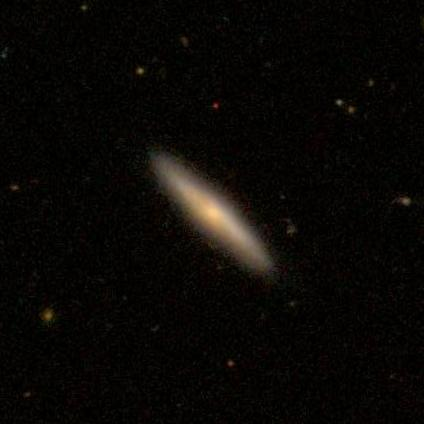
\includegraphics[scale=0.3]{figs/galaxies/elliptical.jpg}}
\caption{Example Images from the Kaggle Galaxy Zoo dataset}
\label{galaxy_examples}
\end{center}
\vskip -0.2in
\end{figure}


Considering this experiment works with using Deep Learning architectures, Kaggle Galaxy Zoo dataset is one of the best datasets available because of the vast size of galaxies. The number of images for each type of galaxy in the Kaggle Galaxy Zoo dataset is provided in Table: \ref{image_numbers}. Also one of the best advantages of this dataset is that the number of images are not highly skewed based on the class labels and are pretty balanced out.

\begin{table}[ht]
\caption{Number of Images in the Kaggle Galaxy Zoo Dataset}
\label{image_numbers}
\vskip 0.15in
\begin{center}
\begin{small}
\begin{sc}
\begin{tabular}{lcr}
\toprule
Galaxy Class & Number of Images \\
\midrule
Spiral    & 34105 \\
Elliptical & 25868\\
\bottomrule
\end{tabular}
\end{sc}
\end{small}
\end{center}
\vskip -0.1in
\end{table}


The evaluation metric for this experiment is the accuracy of the cluster assignments of each galaxy image where the cluster assignments are calculated based upon the dominant class label in the various clusters formed.

%%%%%%%%%%%%%%%%%%%%%%%%%%%%%%%%%%%%%%%%%%%%%%%%%%%%%%%%%%%%%%%%%%%%%%%
%%%%%%%%%%%%%%%%%%%%%%%%%%%%%%%%%%%%%%%%%%%%%%%%%%%%%%%%%%%%%%%%%%%%%%%












%%%%%%%%%%%%%%%%%%%%%%%%%%%%%%%%%%%%%%%%%%%%%%%%%%%%%%%%%%%%%%%%%%%%%%%
% Related Work %
%%%%%%%%%%%%%%%%%%%%%%%%%%%%%%%%%%%%%%%%%%%%%%%%%%%%%%%%%%%%%%%%%%%%%%%
\section{Related Work}

Classification of the galaxy images is one of the most common research topic that is widely studied for solving the problem of understanding the underlying structures in galaxies and trying to solve the problem of label collection for new galaxy images collected by the telescopes every minute. The task of galaxy image classification has been studies for quite some time and traditionally has relied on sophisticated machine learning techniques which depend on extracting useful features from the images and their metadata based on the physical feature information for the galaxy collected by the telescopes. 


\subsection{Feature Selection and Extraction}
One of the earliest research for galaxy classification by Storrie-Lombardi `et~al.' \cite{13_features} found out 13 most important features based on the datasets and used these features as the input features to different architectures of a simple Artificial Neural Network (ANN). Another team used similarly extracted features from the galaxy dataset but implemented a Decision Tree algorithm \cite{dt} for classifying the galaxies. Considering the high dimensionality of pixel level image data and the performance of machine learning algorithms through extracted/learned/selected features a lot of research was done in the field of learning better and lower dimensional features from the image data that are better able to classify the galaxy data. 

Past work has been done which uses principal component analysis (PCA) to project the dataset to a lower dimensionsional space and use the features from the lower dimensional space as the inputs to ANN and locally weighted regression \cite{nn_pca_lwr}. Another research study \cite{nn_pca} employs a similar technique where the extract some latent features in an automated matter and use them in conjunction with PCA learned features as the input features to an ANN for the classification purpose. Other work has also been done in using ensemble methods with ANNs, Decision trees and Naive Bayes Classifiers over the PCA learned feature space \cite{ensembles}. Apart from using PCA learned features several sophisticated features like Gini Coefficients \cite{gini}, optical spectrum of the light rays collected through the telescopes \cite{optical_spectrum} and fourier transforms of the image features \cite{fourier_pca} were developed as input feature vectors to ANN for galaxy classification. Apart from focusing on feature engineering from the galaxy images research was also done on using the image pixels as direct inputs to deeper and larger ANN architecture \cite{ann_geometric_ann_image}. The research explored how well do ANNs learn distinguishing features from the image pixel values. 

It is important to note that almost all of these methods focused on feature learning and selection for finding the input vector for machine learning algorithms or ANNs. This was the primary concern for all of these research groups because of the lack of better algorithms as image processing deep learning architectures, i.e. CNN hadnt been developed yet. Also it was not easy to train very large and deep ANNs because of the lack of especially designed hardware. 

\subsection{Convolutional Neural Networks}
Convolutional Neural Networks (CNN) were designed specifically for the purpose of processing visual data like images. In today’s time, CNN based architectures have been widely used in fields like Image Classification \cite{imagenet} and Object Detection. The motivating idea behind CNNs is that visual data has an inherent local structure such that values which are closer to each other tend to influence each other \cite{cnn}. To understand this, we can take the example of an image of a scenery. We know pixels representing the grass in the image tend to be similar to each other (mostly green). CNNs are very powerful tool because they automatically learn different latent visual features also termed as ”feature maps” from the input image. This property makes CNN’s very different from other traditional Machine Learning Algorithms, where the features have to be already specified. Considering that CNNs learn these high dimensional feature maps from the given input research has been conducted on using these deep CNN networks for directly classifying the galaxy image data \cite{khan}. In their work, a pretrained CNN network: \textbf{``Xception Network"} \cite{xception} was trained using greedy layerwise training for galaxy classification over the Sloan Digital Sky Survey (SDSS) and Dark Energy Survey (DES) dataset. They have shown very high accuracy is achieved by using such network over this task for both training and test sets.

\subsection{Galaxy Zoo Data Classification - Kaggle}
The Kaggle Galaxy Zoo Dataset is the official dataset of Kaggle's: \textbf{Galaxy Zoo - The Galaxy Challenge}. This competition focused on minimizing the classification loss over all the possible classes for galaxies in the test dataset. The online competition drew a total of $427$ competitors from $326$ teams totaling around $3159$ entries. The winning entry by \textbf{Sander Dieleman} used a CNN architecture with heavy data augmentation as part of the training and testing process. The architectur of the CNN was modified a little bit to exploit the rotation invariance of the images and increase parameter sharing. Considering that CNNs are very privy to overfitting the data, regularization for the parameters was implemented in the model by using Dropout layers \cite{dropout}


Some work has been done in clustering the galaxy image data using CNN \cite{khan}, however the technique used relies on features output by a CNN which is trained to minimize the classiication loss over the galaxy image dataset, and then applying t-SNE algorithm \cite{tsne} to cluster the features in a lower dimensional space. This is different from a basic clustering approach because the features were extracted after training was done, which was supervised, while clustering is supposed to be completely unsupervised. 
%%%%%%%%%%%%%%%%%%%%%%%%%%%%%%%%%%%%%%%%%%%%%%%%%%%%%%%%%%%%%%%%%%%%%%%
%%%%%%%%%%%%%%%%%%%%%%%%%%%%%%%%%%%%%%%%%%%%%%%%%%%%%%%%%%%%%%%%%%%%%%%

















%%%%%%%%%%%%%%%%%%%%%%%%%%%%%%%%%%%%%%%%%%%%%%%%%%%%%%%%%%%%%%%%%%%%%%%
% Approach %
%%%%%%%%%%%%%%%%%%%%%%%%%%%%%%%%%%%%%%%%%%%%%%%%%%%%%%%%%%%%%%%%%%%%%%%
\section{Approach}

For this experiment we propose a more complex architecture that connects a pretrained CNN network to the DEC architecture. The main idea behind this network architecture is that CNNs are better suited for extracting features from images as compared to simple ANN model. We are using a pretrained networks because this way we are able to avoid training very large networks which takes a lot of time, computation power and training data. Also pretrained models have been proven very effective in extracting useful features from the images which can be fine tuned for the current problem using transfer learning \cite{transfer_learning}. 


\subsection{Xception Architecture}
For our network architecture we are primarily focusing on using the Xception \cite{xception} network pretrained on the ILSVRC Challenge \cite{imagenet}. The Xception Network can be referred to in Figure: \ref{figure_xception}

\begin{figure}[ht]
\vskip 0.2in
\begin{center}
\centerline{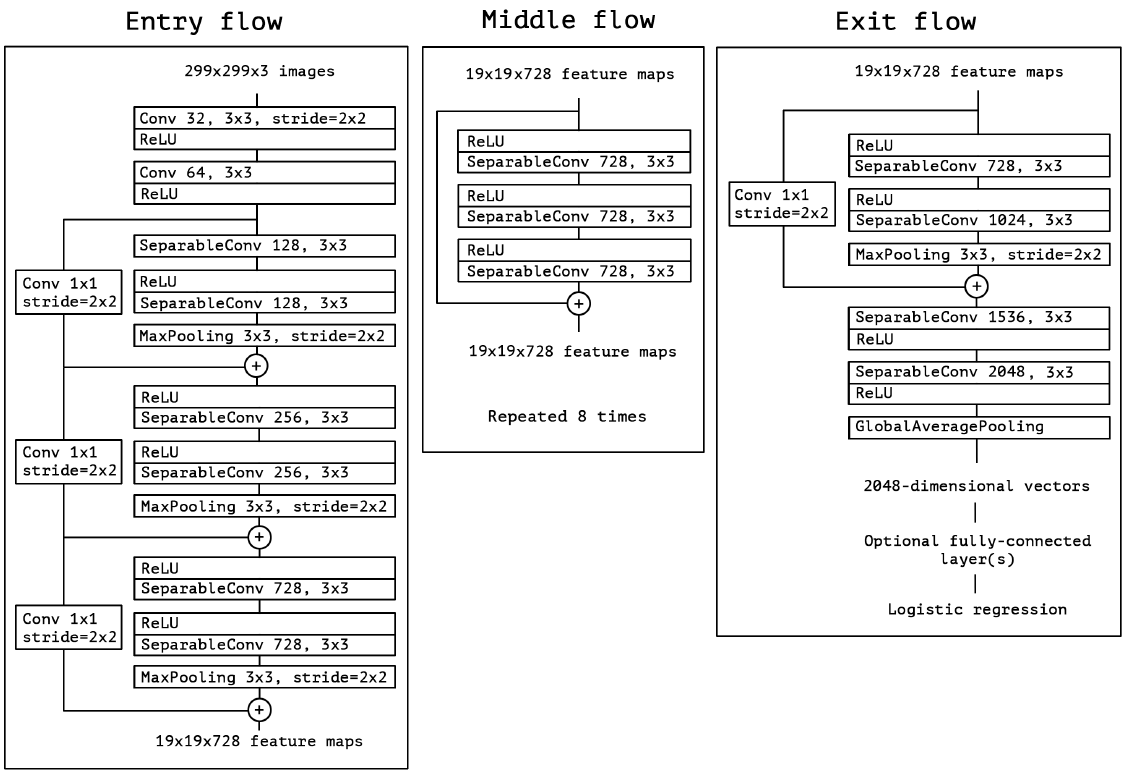
\includegraphics[width=\columnwidth]{figs/xception.png}}
\caption{Xception Network Architecture}
\label{figure_xception}
\end{center}
\vskip -0.2in
\end{figure}

Xception architecture was proposed by Google as a modification of the original Inception network, such that it includes Depthwise Separable Convolutions. Deptwise Separable Convolutions help in reducing the number of opertaions it takes for a convolutional filter to move from an input feature space to an output feature space. It is able to achieve this by dividing a convolution into 2 sequential steps: Depthwise Convolution and Pointwise Convolution. Depthwise convolution (figure: \ref{figure_depthwise}) as the name suggests transforms the input image tensor into an intermediate output tensor that has the desired spatial dimensions but the same depth (number of channels). After the depthwise convolution, pointwise convolution (figure: \ref{figure_pointwise}) transforms this intermediate image tensor and change its number of channels to match the final output image tensor shape using a 1X1 convolution which help preserve the spatial dimensions of the intermediate image tensor (same as output image tensor).

\begin{figure}[ht]
\vskip 0.2in
\begin{center}
\centerline{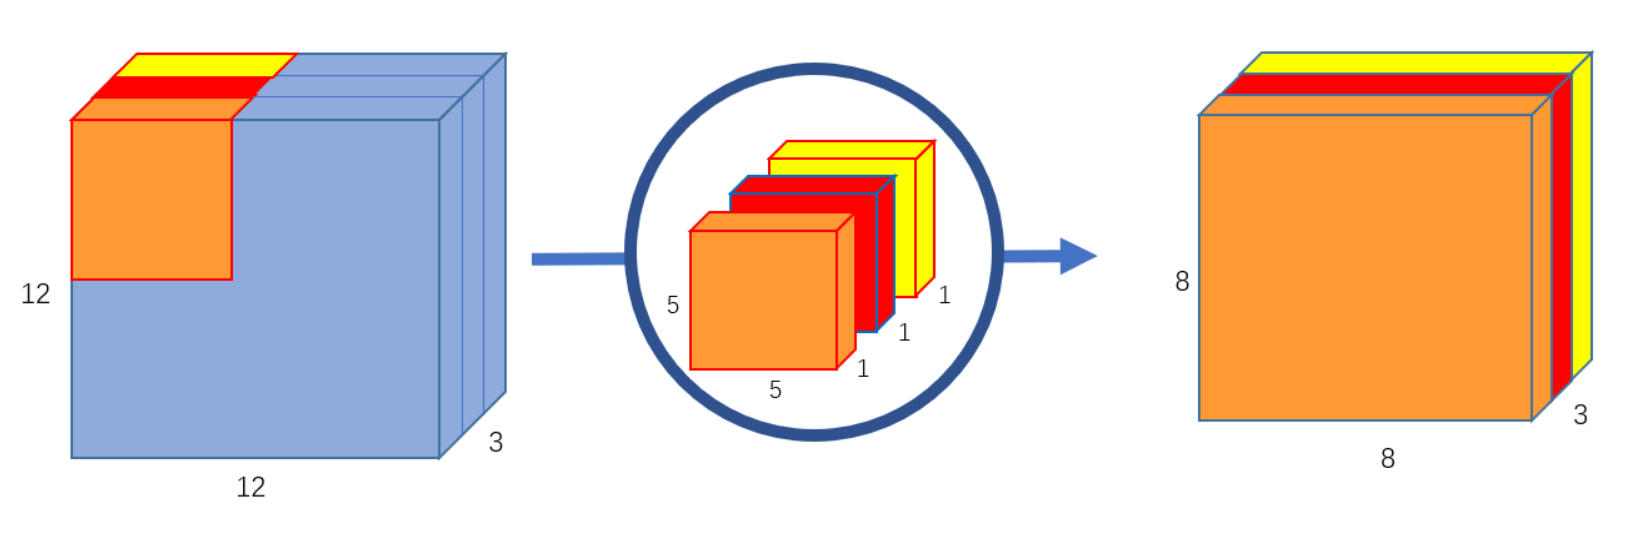
\includegraphics[width=\columnwidth]{figs/depthwise.png}}
\caption{Depthwise Convolution}
\label{figure_depthwise}
\end{center}
\vskip -0.2in
\end{figure}

\begin{figure}[ht]
\vskip 0.2in
\begin{center}
\centerline{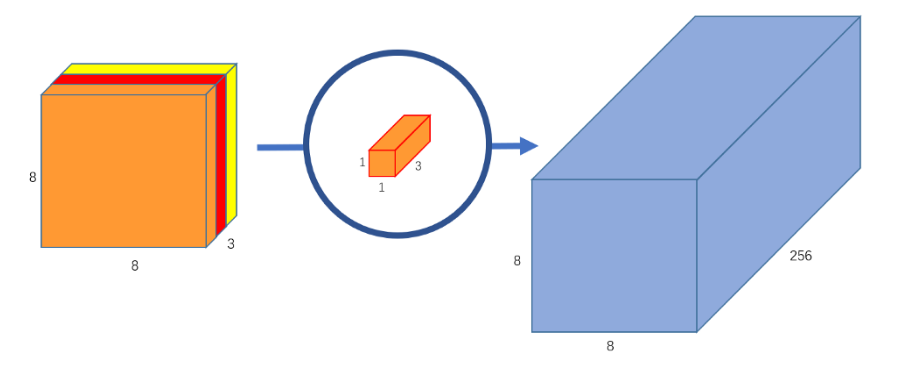
\includegraphics[width=\columnwidth]{figs/pointwise.png}}
\caption{Pointwise Convolution}
\label{figure_pointwise}
\end{center}
\vskip -0.2in
\end{figure}

By employing these techniques the number of parameters decrease in the network, because of smaller size of the convolutions and lower number of convolution filters, without any deviation from the original transformation. Because of the decrease in number of parameters, the number of operations it takes for the transformation also decreases thus leading to a more efficient network. It has been proven that Depthwise Separable Convolutions is able to achieve similar or sometimes even better accuracy on the ILSVRC dataset over the preexisting networks because of the efficient use of the model parameters \cite{xception}.


\subsection{Deep Embedding Clustering}
Because Zooniverse, uses a clustering algorithm to speed up the label collection for the galaxies, this experiment uses Deep Embedding Clustering \cite{dec}: an ANN based architecture that performs clustering on the input feature space as the clustering algorithm attached to the Xception CNN network. The DEC architecture can be visualized in Figure: \ref{figure_dec}. 

\begin{figure}[ht]
\vskip 0.2in
\begin{center}
\centerline{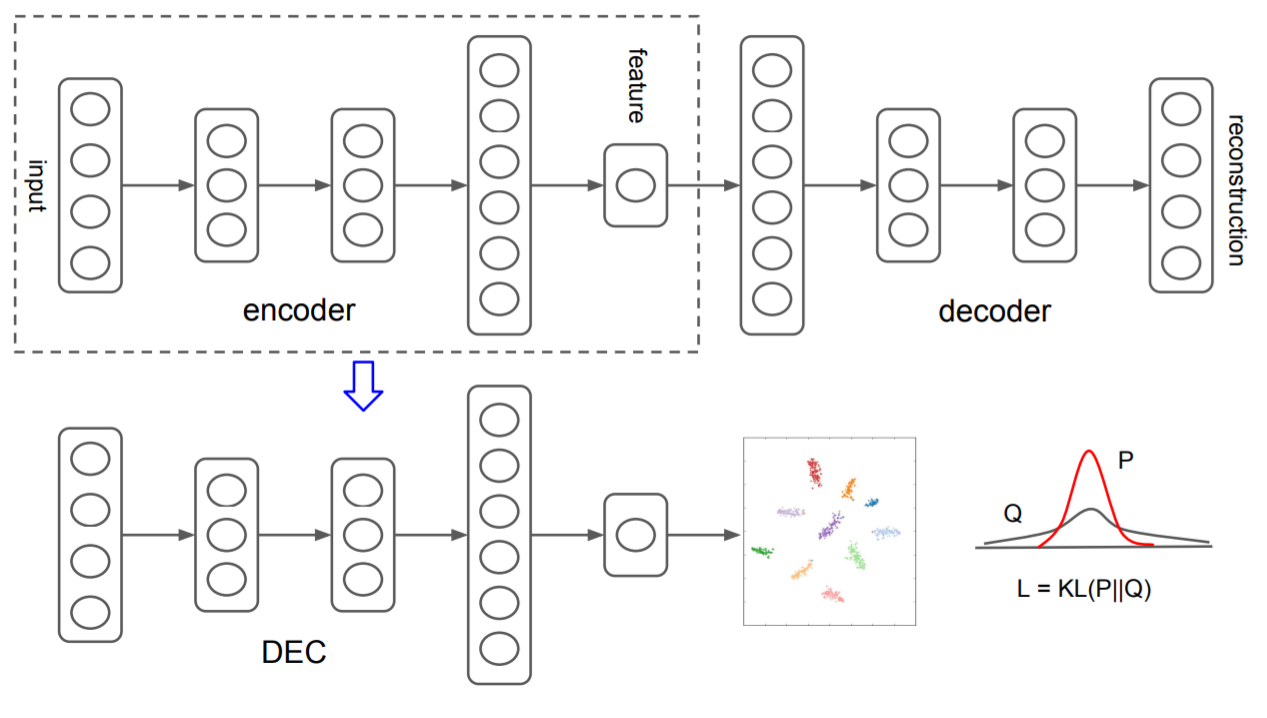
\includegraphics[width=\columnwidth]{figs/dec.png}}
\caption{Deep Embedding Clustering Network Architecture}
\label{figure_dec}
\end{center}
\vskip -0.2in
\end{figure}


The DEC network training for clustering can be divided into two steps as follows:

\subsubsection{Feature Extraction}
The initial step of DEC is to convert the input feature space into a lower dimensional feature space using an ANN stacked autoencoder network. The stacked autoencoder network is constructed using layer wise denoising autoencoder and training them greedily for each denoising autoencoder to reduce the reconstruction loss on the output of the previous denoising autoencoder network. A denoising autoencoder is a simple 2 layer neural network defined using equations \eqref{eq_denoising_autoencoder}

\begin{equation}
\begin{aligned} 
\tilde{x} & \sim \operatorname{Dropout}(x) \\ 
h &= g_{1}\left(W_{1} \tilde{x}+b_{1}\right) \\ 
\tilde{h} & \sim \operatorname{Dropout}(h) \\ 
y &=g_{2}\left(W_{2} \tilde{h}+b_{2}\right) 
\end{aligned}
\label{eq_denoising_autoencoder}
\end{equation}

Here $x$ is the features learned from the previous autoencoder, $Dropout(.)$ \cite{dropout} is a stochastic
mapping that randomly sets a portion of its input dimensions to 0, $g_1$ and $g_2$ are activation functions for encoding
and decoding layer respectively, and $\theta=\left\{W_{1}, b_{1}, W_{2}, b_{2}\right\}$
are model parameters. Training is performed by minimizing the Reconstruction loss which is given by equation \eqref{eq_reconstruction_loss}.

\begin{equation}
\begin{aligned} 
\|x-y\|_{2}^{2}
\end{aligned}
\label{eq_reconstruction_loss}
\end{equation}

By training the stacked autoencoder network, we are able to learn the weights for the encoder which is able to succesfully reduce the dimensionality of the input feature space and project it to a lower dimensional space which is still capable of reconstructing the original features.

\subsubsection{Clustering}
After the initial step of learning the weights of the encoder to project the features to a lower dimensional space, the architecture uses the K-Means Clustering algorithm to cluster the encoded features and find the initial cluster center over the single pass of the whole dataset through the encoder. After that the network's weights and the cluster centers are updated using a gradient descent method which tries to minimize the K-L divergence \cite{kl_divergence}. The weights update rule for the encoder features is given in equation \eqref{eq_feature_update}, and the update rule for the clusters center is given in equation \eqref{eq_cluster_center_update}.

\begin{equation}
\begin{aligned} \frac{\partial L}{\partial z_{i}} &=\frac{\alpha+1}{\alpha} \sum_{j}\left(1+\frac{\left\|z_{i}-\mu_{j}\right\|^{2}}{\alpha}\right)^{-1} \\ & \times\left(p_{i j}-q_{i j}\right)\left(z_{i}-\mu_{j}\right) \end{aligned}
\label{eq_feature_update}
\end{equation}


\begin{equation}
\begin{aligned} \frac{\partial L}{\partial \mu_{j}}=&-\frac{\alpha+1}{\alpha} \sum_{i}\left(1+\frac{\left\|z_{i}-\mu_{j}\right\|^{2}}{\alpha}\right)^{-1} \\ & \times\left(p_{i j}-q_{i j}\right)\left(z_{i}-\mu_{j}\right) \end{aligned}
\label{eq_cluster_center_update}
\end{equation}

Here $z_i$ are the encoder features, $q_{ij}$ is the probability of $z_i$ belonging to $\mu_j$, and $p_{ij}$ is auxiliary distribution based probability of $z_i$ belonging to $\mu_j$. The gradients $\partial L / \partial z_{i}$ are then passed down to the encoder network and used in standard backpropagation to compute the parameter gradient $\partial L / \partial \theta$. This step is repeated until the number of points that change their cluster assignments is below a certain user defined threshold.
%%%%%%%%%%%%%%%%%%%%%%%%%%%%%%%%%%%%%%%%%%%%%%%%%%%%%%%%%%%%%%%%%%%%%%%
%%%%%%%%%%%%%%%%%%%%%%%%%%%%%%%%%%%%%%%%%%%%%%%%%%%%%%%%%%%%%%%%%%%%%%%



















%%%%%%%%%%%%%%%%%%%%%%%%%%%%%%%%%%%%%%%%%%%%%%%%%%%%%%%%%%%%%%%%%%%%%%%
% Experiment %
%%%%%%%%%%%%%%%%%%%%%%%%%%%%%%%%%%%%%%%%%%%%%%%%%%%%%%%%%%%%%%%%%%%%%%%
\section{Experiment}
Before evaluating the performance of the architecture on the task of clustering the galaxies, we also evaluate the proposed architecture on the classification task of the image using a fully supervised training regime. This experiment is conducted to evaluate the performance of the architecture as compared to other past architectures. Apart from supervised training, several experiments were conducted for evaluating the clustering performance of the architecture. Experiments included using different image preprocessing techniques, different architectures of the DEC stacked autoencoder, using different clustering algorithms for the cluster initialization, manually initializing the clusters using labels from the dataset, semi supervised learning to help converge the model and obtain better clustering accuracy. For all the experiments except where discussed, we use the default stacked autoencoder architecture dimensions to 2048-500-500-2000-10 \cite{dec}, along with the number of clusters as 2 which is equal to the number of target classes. The first layer of the network architecture is a 2048 dimensional because it corresponds to the size of the features extracted from the Xception network.

All of the experiments were conducted using code written in python with backend libaries like: tensorflow, keras, numpy, pandas, cv2, matplotlib, seaborn etc. We used ipython notebooks to conduct the experiments because of their ease of access for data analysis. The experiments for this project can be broken into 6 categories, which are discussed in detail. 


\subsection{Supervised Learning - Classification}
We perform an experiment using Supervised Learning for classification of the galaxy images using a simple ANN network and also a CNN network using the Xception network architecture. The experiments for the supervised learning also includes changing the architecture of the ANN (fully connected layers at the end of the network). We perform this experiment to fgure out the best possible performance on the dataset and use this as a reference for the best performance that our unsupervised algorithm can achieve. The fully connected layers in the ANN and CNN network use \textbf{ReLU} ((INSERT REFERENCE)) activation \eqref{eq_relu}, except for the output layer which uses \textbf{Sigmoid} activation \eqref{eq_sigmoid} because we are attempting a binary classification problem.

\begin{equation}
\begin{aligned}  f(x)=x^{+}=\max (0, x) \end{aligned}
\label{eq_relu}
\end{equation}


\begin{equation}
\begin{aligned}  S(x)=\frac{1}{1+e^{-x}} \end{aligned}
\label{eq_sigmoid}
\end{equation}

The loss of the network is \textbf{binary crossentropy} \eqref{eq_binary_crossentropy}, and the network is trained using the \textbf{adam} ((INSERT REFERENCE)) optimizer.

\begin{equation}
\begin{aligned}  BCE = \left\{\begin{matrix} & - log(f(s_{1})) & & if & t_{1} = 1 \\ & - log(1 - f(s_{1})) & & if & t_{1} = 0 \end{matrix}\right. \end{aligned}
\label{eq_binary_crossentropy}
\end{equation}

where $s_1$ is the output of the network after applying the sigmoid activation, and $t_1$ is the true class label.

\subsection{Data Preprocessing}

For this project we consider 2 different categories of data preprocessing.

\subsubsection{Image Preprocessing}
Considering that our input data is galaxy images of size 424 by 424 pixels, we use different image preprocessing techniques to reduce the dimensions of the image to avoid curse of high dimensionality. We reduce the size of image by either resizing the images to a lower dimension, or cropping to a smaller part of the image.

\subsubsection{Feature Preprocessing}
As our inputs are galaxy images, the features to the networks are the RGB values of each pixel from the image. The RGB values are integers falling in the range from 0 to 255. 




\subsection{DEC Stacked Autoencoder Architecture}

\subsection{Clustering Algorithm}

\subsection{Cluster Initialization}

\subsection{Semi Supervised Learning}

%%%%%%%%%%%%%%%%%%%%%%%%%%%%%%%%%%%%%%%%%%%%%%%%%%%%%%%%%%%%%%%%%%%%%%%
%%%%%%%%%%%%%%%%%%%%%%%%%%%%%%%%%%%%%%%%%%%%%%%%%%%%%%%%%%%%%%%%%%%%%%%




















%%%%%%%%%%%%%%%%%%%%%%%%%%%%%%%%%%%%%%%%%%%%%%%%%%%%%%%%%%%%%%%%%%%%%%%
% Results %
%%%%%%%%%%%%%%%%%%%%%%%%%%%%%%%%%%%%%%%%%%%%%%%%%%%%%%%%%%%%%%%%%%%%%%%
\section{Results}
%%%%%%%%%%%%%%%%%%%%%%%%%%%%%%%%%%%%%%%%%%%%%%%%%%%%%%%%%%%%%%%%%%%%%%%
%%%%%%%%%%%%%%%%%%%%%%%%%%%%%%%%%%%%%%%%%%%%%%%%%%%%%%%%%%%%%%%%%%%%%%%























%%%%%%%%%%%%%%%%%%%%%%%%%%%%%%%%%%%%%%%%%%%%%%%%%%%%%%%%%%%%%%%%%%%%%%%
% Analysis %
%%%%%%%%%%%%%%%%%%%%%%%%%%%%%%%%%%%%%%%%%%%%%%%%%%%%%%%%%%%%%%%%%%%%%%%
\section{Analysis}
%%%%%%%%%%%%%%%%%%%%%%%%%%%%%%%%%%%%%%%%%%%%%%%%%%%%%%%%%%%%%%%%%%%%%%%
%%%%%%%%%%%%%%%%%%%%%%%%%%%%%%%%%%%%%%%%%%%%%%%%%%%%%%%%%%%%%%%%%%%%%%%

















%%%%%%%%%%%%%%%%%%%%%%%%%%%%%%%%%%%%%%%%%%%%%%%%%%%%%%%%%%%%%%%%%%%%%%%
% Conclusion %
%%%%%%%%%%%%%%%%%%%%%%%%%%%%%%%%%%%%%%%%%%%%%%%%%%%%%%%%%%%%%%%%%%%%%%%
\section{Conclusion}
%%%%%%%%%%%%%%%%%%%%%%%%%%%%%%%%%%%%%%%%%%%%%%%%%%%%%%%%%%%%%%%%%%%%%%%
%%%%%%%%%%%%%%%%%%%%%%%%%%%%%%%%%%%%%%%%%%%%%%%%%%%%%%%%%%%%%%%%%%%%%%%


















%%%%%%%%%%%%%%%%%%%%%%%%%%%%%%%%%%%%%%%%%%%%%%%%%%%%%%%%%%%%%%%%%%%%%%%
% Bibliography %
%%%%%%%%%%%%%%%%%%%%%%%%%%%%%%%%%%%%%%%%%%%%%%%%%%%%%%%%%%%%%%%%%%%%%%%
\bibliography{goelx029_csci5512_project}
\bibliographystyle{icml2019}
%%%%%%%%%%%%%%%%%%%%%%%%%%%%%%%%%%%%%%%%%%%%%%%%%%%%%%%%%%%%%%%%%%%%%%%
%%%%%%%%%%%%%%%%%%%%%%%%%%%%%%%%%%%%%%%%%%%%%%%%%%%%%%%%%%%%%%%%%%%%%%%


















%%%%%%%%%%%%%%%%%%%%%%%%%%%%%%%%%%%%%%%%%%%%%%%%%%%%%%%%%%%%%%%%%%%%%%%
% Appendix %
%%%%%%%%%%%%%%%%%%%%%%%%%%%%%%%%%%%%%%%%%%%%%%%%%%%%%%%%%%%%%%%%%%%%%%%
\appendix
\section{Appendix}
%%%%%%%%%%%%%%%%%%%%%%%%%%%%%%%%%%%%%%%%%%%%%%%%%%%%%%%%%%%%%%%%%%%%%%%
%%%%%%%%%%%%%%%%%%%%%%%%%%%%%%%%%%%%%%%%%%%%%%%%%%%%%%%%%%%%%%%%%%%%%%%



\end{document}

















%% Example of figure:


%% Example of algorithm
%\begin{algorithm}[tb]
%   \caption{Bubble Sort}
%   \label{alg:example}
%\begin{algorithmic}
%   \STATE {\bfseries Input:} data $x_i$, size $m$
%   \REPEAT
%   \STATE Initialize $noChange = true$.
%   \FOR{$i=1$ {\bfseries to} $m-1$}
%   \IF{$x_i > x_{i+1}$}
%   \STATE Swap $x_i$ and $x_{i+1}$
%   \STATE $noChange = false$
%   \ENDIF
%   \ENDFOR
%   \UNTIL{$noChange$ is $true$}
%\end{algorithmic}
%\end{algorithm}


% Note use of \abovespace and \belowspace to get reasonable spacing
% above and below tabular lines.
%\begin{table}[t]
%\caption{Classification accuracies for naive Bayes and flexible
%Bayes on various data sets.}
%\label{sample-table}
%\vskip 0.15in
%\begin{center}
%\begin{small}
%\begin{sc}
%\begin{tabular}{lcccr}
%\toprule
%Data set & Naive & Flexible & Better? \\
%\midrule
%Breast    & 95.9$\pm$ 0.2& 96.7$\pm$ 0.2& $\surd$ \\
%Cleveland & 83.3$\pm$ 0.6& 80.0$\pm$ 0.6& $\times$\\
%Glass2    & 61.9$\pm$ 1.4& 83.8$\pm$ 0.7& $\surd$ \\
%Credit    & 74.8$\pm$ 0.5& 78.3$\pm$ 0.6&         \\
%Horse     & 73.3$\pm$ 0.9& 69.7$\pm$ 1.0& $\times$\\
%Meta      & 67.1$\pm$ 0.6& 76.5$\pm$ 0.5& $\surd$ \\
%Pima      & 75.1$\pm$ 0.6& 73.9$\pm$ 0.5&         \\
%Vehicle   & 44.9$\pm$ 0.6& 61.5$\pm$ 0.4& $\surd$ \\
%\bottomrule
%\end{tabular}
%\end{sc}
%\end{small}
%\end{center}
%\vskip -0.1in
%\end{table}


%Citation
% \cite{Samuel59}.
%%% Multiple Citations
%\cite{kearns89,Samuel59,mitchell80}. Use the 